\documentclass[11pt,letterpaper]{article}
\usepackage[margin=1.0in]{geometry}
\usepackage{amssymb,amsmath,enumerate,mathtools}
\usepackage{graphics,graphicx}
\usepackage{framed, gensymb, listings}

\lstset{
    language=Verilog,                            % sets the language for the code
    basicstyle=\scriptsize\ttfamily,       % for the actual code
    morekeywords={},  % adds keywords
    deletekeywords={if, do, for},               % removes keywords
    keywordstyle=\bfseries,                % for keywords
    commentstyle=\scriptsize\ttfamily,     % for comments 
    showstringspaces=false                 % prevents underscores from appearing in output
}

\begin{document}
\begin{flushright}
Andrew Scott\\
E155\\
Lab 1\\
September 14, 2015
\end{flushright}

\begin{center}
Lab 1: Utility Board Assembly
\end{center}

\textbf{Introduction}\\
In this lab, a utility board was assembled and then tested. The board was then used to power a seven-segment display by writing Verilog code that took input from four switches and displayed the hex number of the binary input from the switches.

\textbf{Design and Testing Methodology}\\
On the hardware side, there were not that many design decisions to be made. I followed the step by step instructions to do all of the soldering, using solder paste for the surface mounts and regular solder wire for the through-hole mounts. For the seven segment display, I decided to bring wires from all of the pins on the display to holes on the breadboard below the display in the order in which their pins appeared on the board. This allowed me to add the resistors and connect to the utility board pins in order (the top utility board pin being used for the display connected to the top resistor/display pin). To test the hardware, I first checked that there were no short circuits in the board by using a multimeter to check the resistance between v$_{\text{in}}$ and ground, and since the resistance was around 0.1 M\ohm I knew there was no short. I then tested the power by hooking the board up to 5V power and checking the voltage on all of the voltage regulators. Finally, I tested the LED's, switches and seven segment display by writing Verilog code and checking that all the outputs from the LED's and the display were the same as they were supposed to be according to the simulation I performed of my Verilog code.

On the software side, there were several design choices to make. I decided to implement the seven segment display control logic as its own module, partly because it was cleaner that way and partly because I will most likely need to use it again in the future and want to have it easily accessible. Another decision I made for the seven segment display was to use some boolean equations for each of the segments that I wrote in E85, which I simplified and were very easy to write in Verilog. The other software design choice I had to make was how to make the last LED flash at 2.4 Hz. I decided to do this using a counter that counted up to a certain number (calculated to be the number of 40 MHz clock cycles in a single 2.4 Hz flash) and then flip the status of the LED every time this number was reached. Although this solution did not feel optimal, I was unsure of any other good way to use the fast clock cycle for something changing as slow as the LED was. To test my software, I ran a simulation in ModelSim and tried every combination of switches, confirming that the output on the LED's was correct. I also tested the seven segment display logic by running the Verilog code on my board and checking that the correct symbol was displayed for each combination of switches pressed. Finally, I timed how long my flashing LED took to flash 10 times, which came out to just over 4 seconds thus showing that it was flashing at around 2.4 Hz.

\textbf{Results and Discussion}\\
I was able to accomplish all of the lab tasks after some debugging. Everything on the board works as it is supposed to. Some of the solder joints are not as pretty as I would like them to be, but this was my first experience with soldering so I am not too disappointed with how the utility board turned out.

\textbf{Conclusion}\\
In this lab I put together a utility board and then used it to control a seven segment display. Everything performed as expected after some debugging. In all, the lab took about 8 hours to complete.


\pagebreak

\textbf{Breadboard Schematic}\\\\
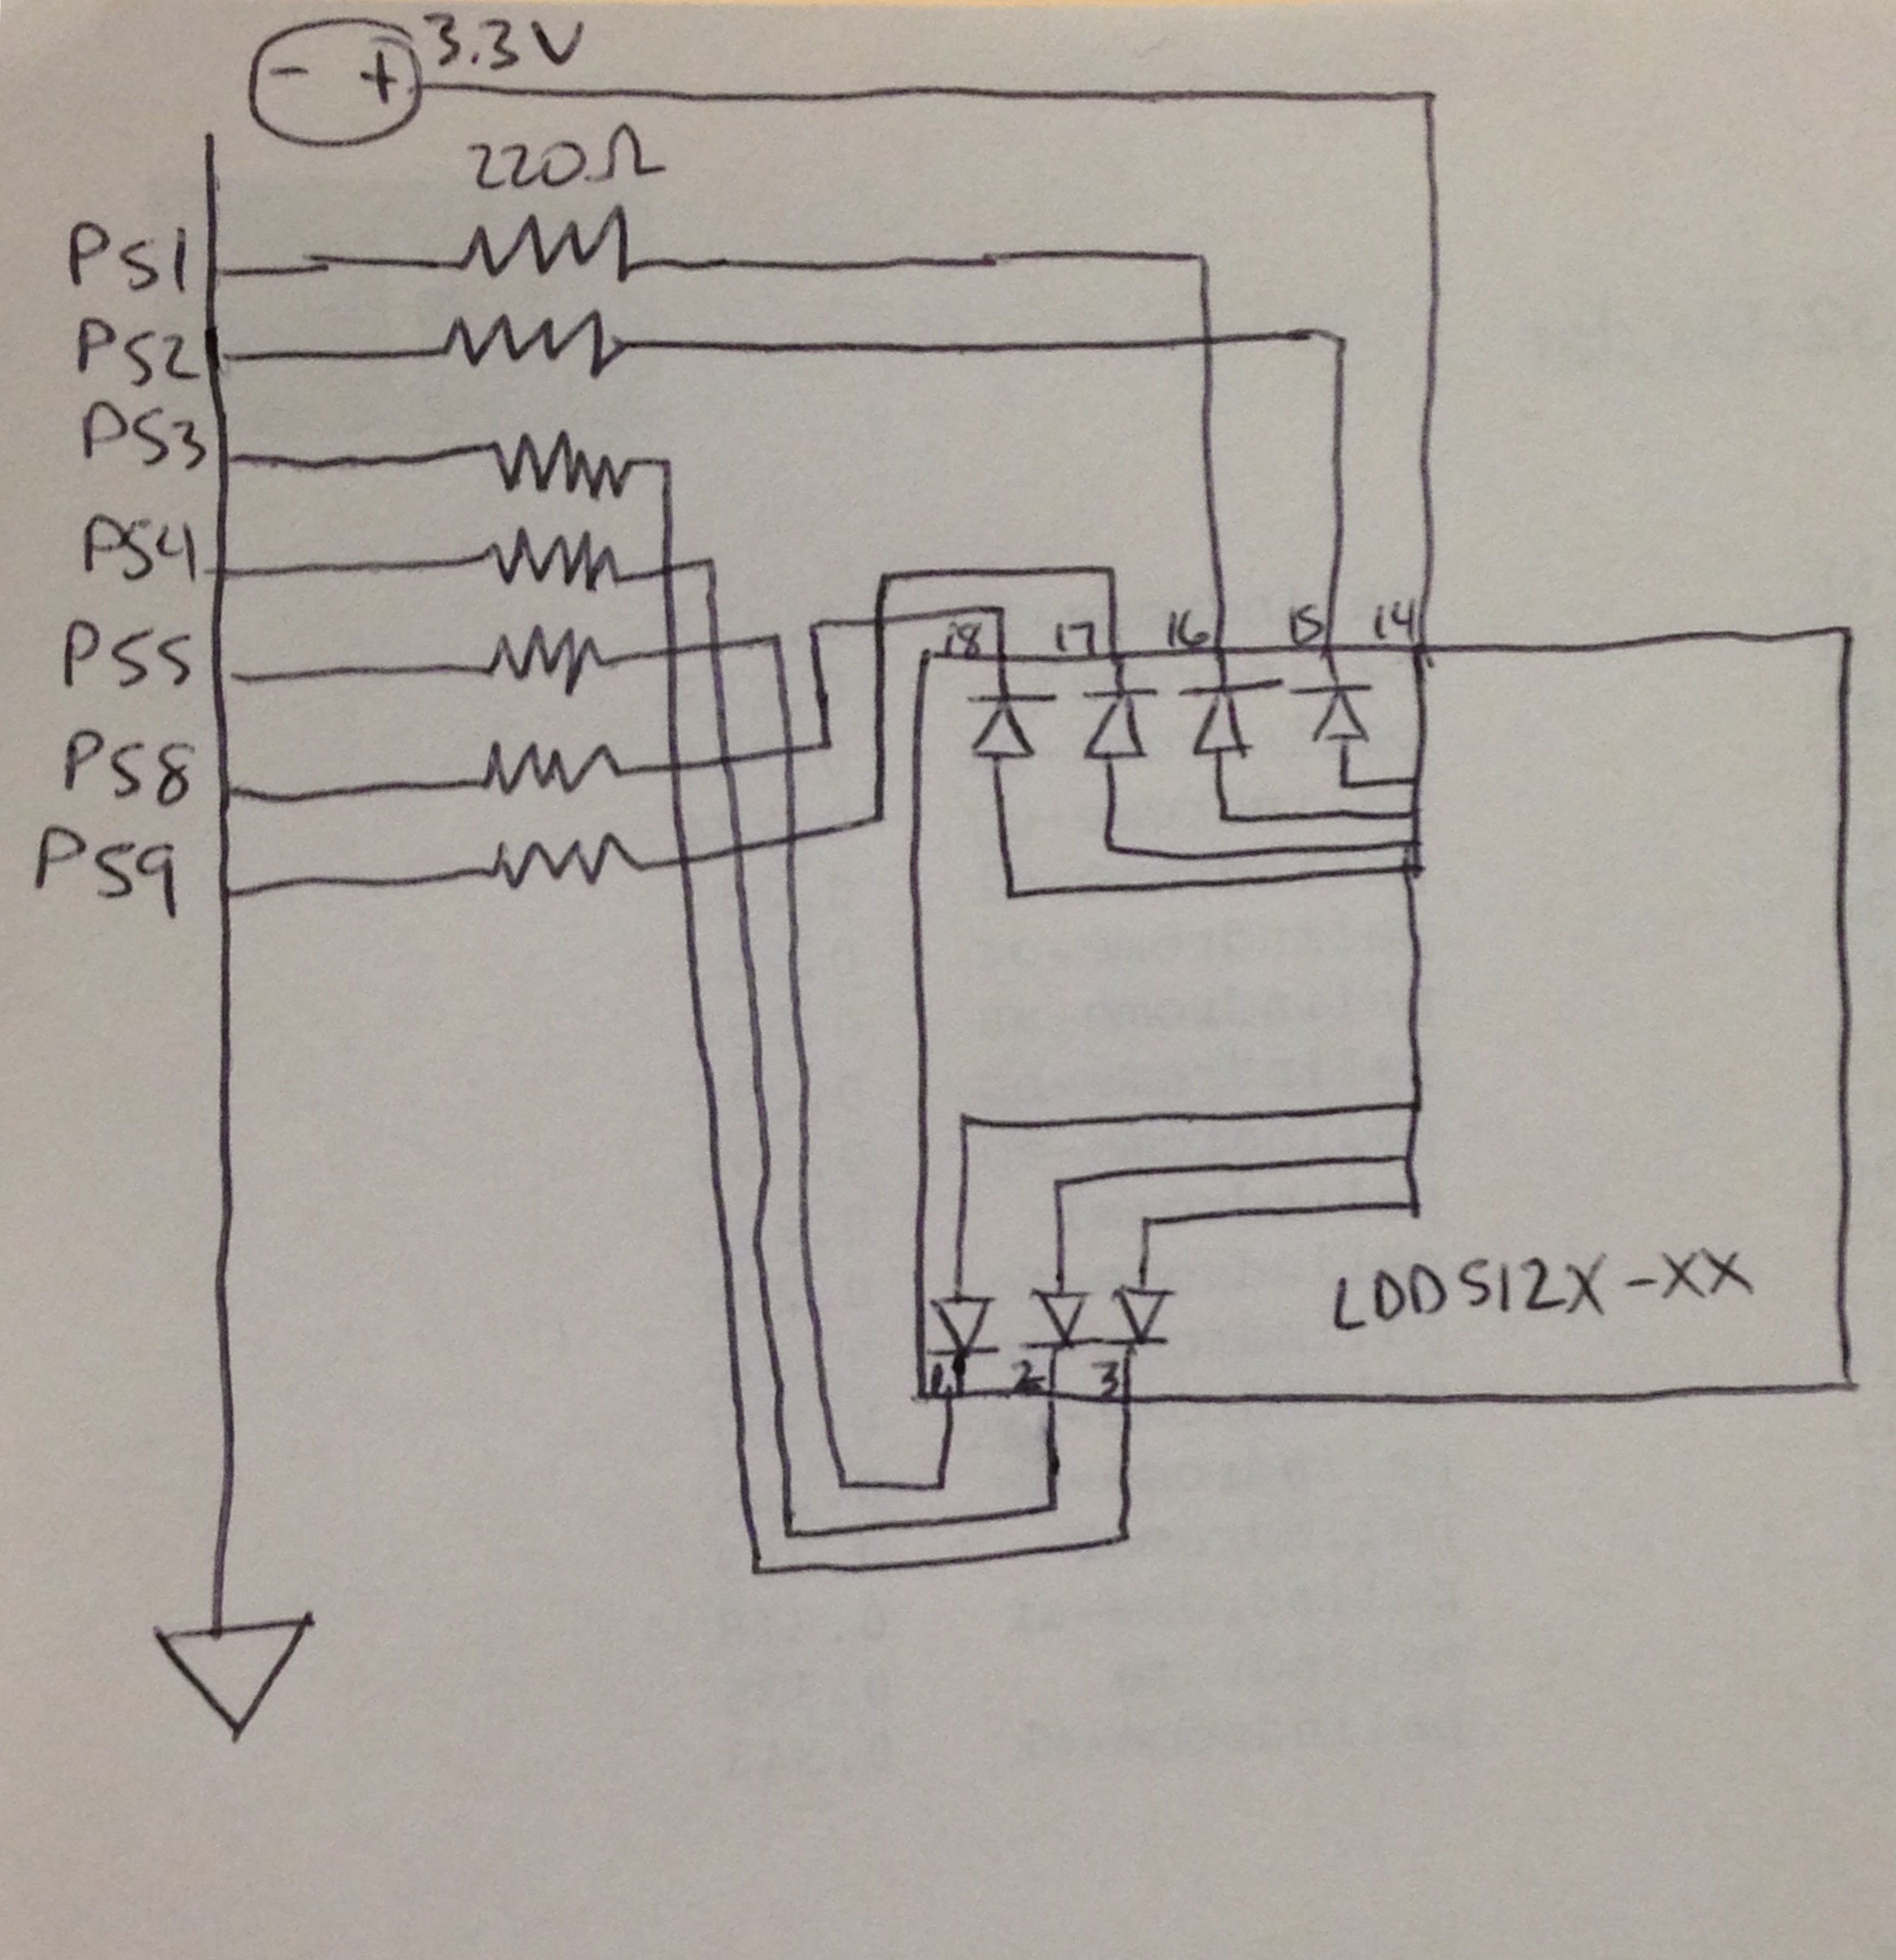
\includegraphics[scale=0.2]{schematic.jpg}

\pagebreak

\textbf{Verilog Code}\\\\
\lstset{language=Verilog}
\lstinputlisting{lab1_as.sv}


\end{document}

